\begin{figure}[t]
    \centering
    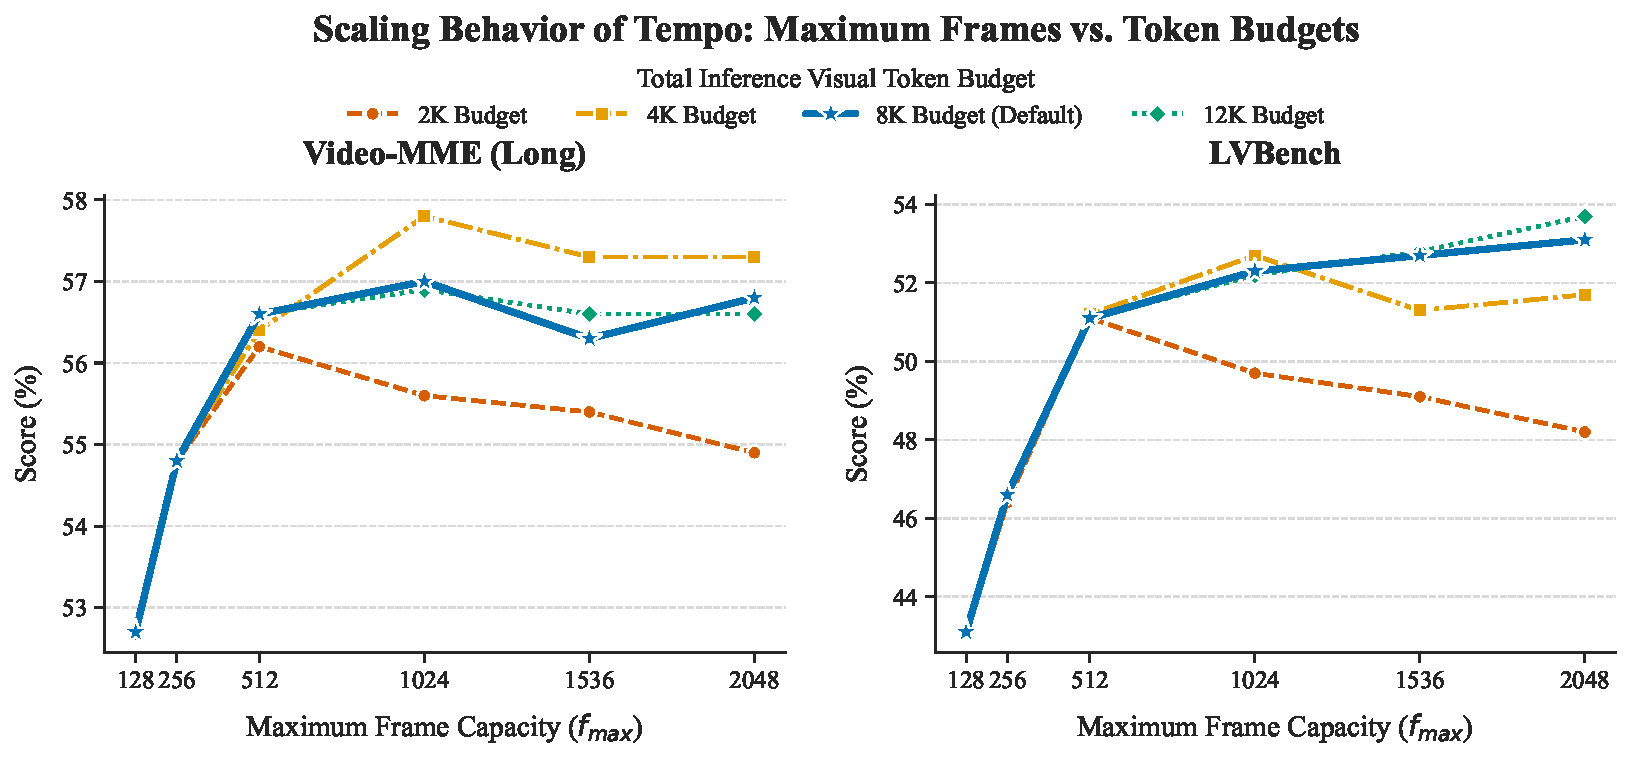
\includegraphics[width=\textwidth]{fig/scaling_behavior.pdf}
    \caption{\textbf{Scaling behavior of Tempo.} We investigate the interplay between maximum frame capacity ($f_{\max}$) and total visual token budgets. \textbf{(Left)} On Video-MME (Long), a strict 4K budget acts as an optimal \emph{sweet spot} by aggressively filtering redundancy, whereas larger budgets (8K/12K) yield marginal noise. \textbf{(Right)} On the extreme-long LVBench, restrictive budgets eventually limit the achievable performance, whereas expansive capacities (\eg, 12K) monotonically unlock new peaks at higher frame densities, proving the necessity of scaled context for hour-long video understanding.}
    % \vspace{-1.5em}
    \label{fig:scaling_behavior}
\end{figure}